\chapter{Modelización de las redes neuronales} \label{ch:modelizacion}

A partir de las herramientas matemáticas que hemos introducido en \customref{ch:matematicas_fundamentales} y de la modelización de la tarea de aprendizaje realizada en \customref{ch:tarea_aprendizaje}, buscamos desarrollar una modelización matemática de las redes neuronales con las que se suele trabajar en la práctica. Para que sea una \textbf{buena modelización}, esta debería cumplir que:

\begin{itemize}
	\item Sea lo más parecida a los modelos que se usan en la práctica.
	\item Permita obtener resultados interesantes.
\end{itemize}

Usando descomposiciones tensoriales, modelaremos dos tipos de redes:

\begin{itemize}
	\item Redes neuronales no profundas, a partir de la descomposición \textit{CANDECOMP/PARAFAC} o descomposición \textit{CP}.
	\item Redes convolucionales profundas, a partir de la descomposición jerárquica de \textit{Tucker} o descomposición \textit{HT} por sus siglas en inglés.
\end{itemize}

Las \textbf{modelizaciones son muy cercanas a las arquitecturas usadas en la práctica del aprendizaje automático}. Principalmente, porque tienen en cuenta las tres propiedades características de una red convolucional:

\begin{enumerate}
	\item Localidad.
	\item Compartición de parámetros, que junto a la localidad, da lugar a la convolución.
	\item \textit{Pooling}.
\end{enumerate}
\todo{Desarrollar de forma más extensa qué significan estas propiedades. Antes digo que voy a explicar qué son estas propiedades. Y además, estoy repitiendo el listado, por lo que tengo que desarrollar bien estas propiedades}

\section{Modelo \textit{CP}}

Este modelo será el resultado de aplicar la descomposición tensorial \textit{CP} en la función de puntuación dada por \eqref{eq:puntuacion_general}. Como veremos más adelante, esto resultará en un modelo \textit{shallow}, con una única capa convolucional oculta.

\subsection{Descomposición CANDECOMP/PARAFAC} \label{subs:descomposcion_cp}

En esta sección introduciremos la descomposición tensorial \textit{CANDECOMP/PARAFAC}. Esta es la descomposición más sencilla de las dos descomposiciones que vamos a manejar. Empecemos introduciendo la siguiente propiedad sobre los tensores puros:

\begin{proposicion}[Rango matricial de los tensores puros]
	Sean $\nv{v} \in \R^{N}, \nv{w} \in \R^{M}$ dos vectores. Entonces su producto tensorial puede expresarse como:

	$$\nv{v} \otimes \nv{w} = \nv{v} \nv{w}^T \in \espaciomatrices{N}{M}$$

	Además, esta matriz es de rango uno o cero (este último caso ocurre únicamente cuando alguno de los dos vectores es $\vec{0}$)
\end{proposicion}

\begin{proof}

	Sean $\nv{v} = (v_1, \ldots, v_N)$ y $\nv{w} = (w_1, \ldots, w_M)$ dos vectores cualesquiera. Entonces, usando la expresión del producto tensorial que introducimos en \customref{sec:otra_forma_tensores}, tenemos que:

	\begin{equation}
		\nv{v} \otimes \nv{w} = (v_i w_j)_{i \in \deltaset{N},\ j \in \deltaset{M}}
	\end{equation}

	O lo que es lo mismo:

	\begin{equation}
		\nv{v} \otimes \nv{w} = \begin{pmatrix}
			v_1 w_1 & v_1 w_2 & \ldots & v_1 w_M \\
			v_2 w_1 & v_2 w_2 & \ldots & v_1 w_M \\
			\vdots  & \vdots  &        & \vdots  \\
			v_N w_1 & v_N w_2 & \ldots & v_N w_M \\
		\end{pmatrix}
	\end{equation}

	Que claramente se corresponde con la expresión de $\nv{v} \nv{w}^T$. Además, es claro que la fila $i$-ésima viene dada por el vector fila

	$$(v_i w_1, v_i w_2, \ldots, v_i w_M) = v_i (w_1, \ldots, w_M) = v_i \nv{w}^T$$

	Por tanto, todas las filas son combinación lineal de una de las filas.

	En el caso de que alguno de los dos vectores $\nv{v}$ o $\nv{w}$ sea $\vec{0}$, tenemos que la matriz $\nv{v} \otimes \nv{w}$ es la matriz de ceros, y por tanto su rango es cero.

	Estudiado ese caso, ahora podemos suponer que $\nv{v}, \nv{w} \neq \vec{0}$, y por tanto se debe cumplir que $\exists i_0 \in \deltaset{N}: v_{i_0} \neq 0$. Esa será la fila que escogemos para expresar el resto de filas como combinación lineal de esta, aprovechando de que es no nula. Dicha fila se puede expresar como $v_{i_0} \nv{w}^T$. La fila $i$-ésima se puede expresar como $v_i \nv{w}^T$. Y por tanto:

	\begin{equation}
		\begin{split}
			v_i \nv{w}^T = \lambda \cdot v_{i_0} \nv{w}^T \iif & \lambda = \frac{v_i}{v_{i_0}} \\
			& \lambda \neq 0 \iif v_i \neq 0
		\end{split}
	\end{equation}

	Con esto sabemos que $rank(\nv{v} \otimes \nv{w}) \leq 1$, pero podría darse el caso de que el rango fuese cero aún siendo $\nv{v}, \nv{w} \neq \vec{0}$. Sin embargo, esto no es posible. Como $\nv{v}, \nv{w} \neq \vec{0}$, entonces $\exists i_0 \in \deltaset{N}, \exists j_0 \in \deltaset{M}$ de modo que $v_{i_0}, w_{j_0} \neq 0$. Por tanto, el menor de orden 1 asociado a la fila $i_0$-ésima y columna $j_0$-ésima tiene el valor $v_{i_0} w_{j_0} \neq 0$, y con ello, $rank(\nv{v} \otimes \nv{w}) \geq 1$.

\end{proof}

\begin{observacion}
	Estamos escribiendo la igualdad $\nv{v} \otimes \nv{w} = \nv{v} \nv{w}^T$ sin definir lo que significa la igualdad entre un tensor de orden 2 y una matriz. Sin embargo, esta igualdad es totalmente natural. Decimos que un tensor de orden dos y una matriz son iguales cuando las dimensiones de la matriz y las dos dimensiones del tensor coinciden, y cuando las entradas de ambos coinciden.
\end{observacion}

La anterior proposición muestra que los tensores puros que vienen dados como producto tensorial de dos vectores tienen un rango matricial igual a uno (en caso de que no sean ambos vectores nulos). Es natural plantearse generalizar esta propiedad a tensores puros que vengan dados como producto tensorial de $N$ vectores. Pero de momento no tenemos una herramienta para comparar tensores de orden $N > 2$ con matrices. Esto motiva la introducción de la descomposición tensorial \textit{CANDECOMP/PARAFAC}:

\begin{proposicion}[\textbf{Descomposición \textit{CANDECOMP/PARAFAC}}]
	Todo tensor $\mathcal{A}$ puede ser expresado como la suma de tensores puros. Es decir, $\forall \mathcal{A} \in \R^{M_1 \times \cdots \times M_N}$, $\exists Z \in \N$:

	\begin{equation} \label{eq:cp_decomp}
		\mathcal{A} = \sum_{i = 1}^Z \nv{v_i^{(1)}} \otimes \cdots \otimes \nv{v_i^{(N)}};
		\qquad \nv{v_i^{(k)}} \in \R^{M_k},
		\dspace \forall i \in \deltaset{Z},
		\dspace \forall k \in \deltaset{N},
	\end{equation}
\end{proposicion}

\begin{observacion}[Origen del nombre de la descomposición]
	En 1927 Hitchcock propone la idea de expresar un tensor como la suma de tensores de rango uno. En 1970 se introducen dos trabajos independientes que resuelven esta tarea. El primero, introducido por Carol y Chang, propone la descomposición canónica (\textit{CANonical DECOMPosition} o \textit{CANDECOMP}). El segundo trabajo, introducido por Harshman, propone la descomposición por factores paralelos (\textit{PARallel FACtors} o \textit{PARAFAC}). Más tarde se descubre que ambas descomposiciones son equivalentes, por lo que se adopta el nombre conjunto \cite{matematicas:cp_nombre_paper}.
\end{observacion}

\begin{observacion}
	Esta descomposición es equivalente a la siguiente descomposición:

	\begin{equation}
		\mathcal{A} = \sum_{i = 1}^Z \lambda_i \cdot \nv{v_i^{(1)}} \otimes \cdots \otimes \nv{v_i^{(N)}};
		\qquad \nv{v_i^{(k)}} \in \R^{M_k},
		\dspace \lambda_i \in \R,
		\dspace \forall i \in \deltaset{Z},
		\dspace \forall k \in \deltaset{N},
		\dspace Z \in \N
	\end{equation}

	Puesto que podemos considerar:

	\begin{equation}
		\nv{w_i^{(1)}} := \lambda_i \cdot \nv{v_i^{(1)}} \in \R^{M_1}
	\end{equation}

	y usando de nuevo las propiedades del producto tensorial:

	\begin{equation}
		\lambda_i \cdot \nv{v_i^{(1)}} \otimes \nv{v_i^{(2)}} \otimes \cdots \otimes \nv{v_i^{(N)}} = \nv{w_i^{(1)}} \otimes \nv{v_i^{(2)}} \otimes \cdots \otimes  \nv{v_i^{(N)}}
	\end{equation}
\end{observacion}

\begin{observacion}
	Nótese que el número de vectores que multiplicamos tensorialmente es constante, no varía dicho número de vectores entre sumandos. Y dicho número coincide con el orden $N$ del tensor que estemos construyendo.
\end{observacion}

% TODO -- seguir por aqui
\begin{proof} \label{proof:demostracion_cp_es_universal}
	Queremos descomponer el tensor $\mathcal{A}$ que tiene orden $N$ y dimensión $M_k$ en cada dimensión $k \in \deltaset{N}$. Por tanto, $\mathcal{A}$ tiene $M_1 M_2 \ldots M_N$ elementos. En base a esto, tomamos $Z = M_1 M_2 \cdots M_N$ y en cada sumando de la descomposición buscamos colocar un único coeficiente del tensor en su índice correspondiente.

	Por tanto, en cada sumando buscamos encontrar vectores cuyo producto tensorial genere un tensor, de dimensiones adecuadas, con todas las entradas nulas salvo la entrada de la que nos ocupamos en esa iteración.

	Para que la demostración sea más clara cambiaremos la forma de indexar la suma. En la proposición estamos usando un único índice que llega hasta $Z = M_1 \cdot \ldots \cdot M_N$. Esto es lo mismo que usar $N$ índices que lleguen hasta $M_k$, y así la sumatoria queda:

	\begin{equation}
		\mathcal{A} = \sum_{d_1 = 1}^{M_1} \sum_{d_2 = 1}^{M_2} \cdots \sum_{d_N = 1}^{M_N} \lambda_{i_1, \ldots, i_N} \cdot \nv{v_{(i_1, \ldots, i_N)}^{(1)}} \otimes \cdots \otimes \nv{v_{(i_1, \ldots, i_N)}^{(N)}}
	\end{equation}

	Para llevar a cabo la idea de usar cada sumando para colocar un elemento de $\mathcal{A}$ en sus índices correctos, haremos que en cada sumando se verifique

	\begin{itemize}
		\item $\lambda_{i_1, \ldots, i_N} = \mathcal{A}_{i_1, \ldots, i_N}$. Esto es inmediato y no necesita más explicación
		\item $\nv{v_{(i_1, \ldots, i_N)}^{(1)}} \otimes \cdots \otimes \nv{v_{(i_1, \ldots, i_N)}^{(N)}}$ genere el tensor en $\R^{M_1 \times \cdots \times M_N}$ que sea cero en todas las entradas salvo en el índice $(i_1, \ldots, i_N)$, donde valdrá 1. Dicho tensor lo podemos denotar como  $\mathcal{B}^{(i_1, \ldots, i_N)}$
	\end{itemize}

	Ahora, veamos cómo podemos generar el tensor $\mathcal{B}^{(i_1, \ldots, i_N)}$ como producto tensorial de ciertos vectores. La propiedad fundamental que queremos que ese tensor cumpla es:

	\begin{equation}
		\mathcal{B}^{(i_1, \ldots, i_N)}_{j_1, \ldots, j_N} =
		\begin{cases}
			1 & \text{si } i_1 = j_1, \ldots, i_N = j_N \\
			0 & \text{en otro caso}
		\end{cases}
	\end{equation}

	Definimos $\nv{\delta_{i, N}}$ como el vector de longitud $N$, con todas las entradas nulas salvo la entrada de la posición $i$, en la que ponemos un uno. Por tanto, es claro que:

	\begin{equation}
		(\nv{\delta_{i, N}})_k =  \delta_{i, k} =
		\begin{cases}
			1 & \text{si } i = k    \\
			0 & \text{en otro caso}
		\end{cases}
	\end{equation}

	Definimos

	\begin{equation}
		\mathcal{B}^{(i_1, \ldots, i_N)} := \nv{\delta_{i_1, M_1}} \otimes \cdots \otimes \nv{\delta_{i_N, M_N}}
	\end{equation}

	y por tanto se verifica que:

	\begin{equation}
		\mathcal{B}^{(i_1, \ldots, i_N)}_{j_1, \ldots, j_N} = (\vec{\delta}_{i_1, M_1})_{j_1} \cdots (\vec{\delta}_{i_N, M_N})_{j_N} = \delta_{i_1, j_1} \cdots \delta_{i_N, j_N} =
		\begin{cases}
			1 & \text{si } i_1 = j_1, \ldots, i_N = j_N \\
			0 & \text{en otro caso}
		\end{cases}
	\end{equation}

	como buscábamos. Y con esto es trivial ver nuestra descomposición:

	\begin{equation}
		\mathcal{A} = \sum_{d_1 = 1}^{M_1} \sum_{d_2 = 1}^{M_2} \cdots \sum_{d_N = 1}^{M_N} \mathcal{A}_{i_1, \ldots, i_N} \cdot \vec{\delta}_{i_1, M_1} \otimes \ldots \otimes \vec{\delta}_{i_N, M_N}
	\end{equation}
\end{proof}


\begin{observacion}[Descomposición conjunta] \label{observacion:descomposicion_cp_conjunta}

	Notar que en la demostración hemos fijado un cojunto de vectores que solo depende del tensor a descomponer en cuanto que tenemos que considerar las dimensiones del tensor. Si fijamos un espacio de tensores, $\R^{M_1 \times \cdots M_N}$, entonces este conjunto de vectores no depende del tensor a descomponer. Es decir, podemos usar estos vectores para descomponer cualquier tensor $\mathcal{A} \in \R^{M_1 \times \cdots \times M_N}$. Este conjunto de vectores es:

	\begin{equation}
		\conjunto{\delta_{k, L}: \; L \in \deltaset{M}, \; k \in \deltaset{L}}
	\end{equation}

	donde $M := \max \conjunto{M_1, \ldots, M_N}$.

\end{observacion}

\begin{observacion}

	En la demostración, hemos tomado $Z = M_1 \cdot \ldots \cdot M_N$ para asegurarnos de la existencia de una tal descomposición. Sin embargo, es razonable pensar que existirán combinaciones de vectores con las que podamos tomar un valor de $Z$ menor. De hecho, buscar una descomposición que minimice el valor de $Z$ es un problema de optimización complejo.

	Esto motivará la siguiente definición.
\end{observacion}

\begin{definicion}[Rango \textit{CP}]
	Dado un tensor $\mathcal{A}$, se define su rango \textit{CP} como el mínimo valor de $Z$ para el cual la ecuación \eqref{eq:cp_decomp} se mantiene

\end{definicion}

Una propiedad interesante es la siguiente:

\begin{proposicion}[]
	Para un tensor de orden dos, que podemos ver como una matriz, su rango \textit{CP} coincide con el rango matricial usual
\end{proposicion}

\subsection{Aplicando la descomposición a la función de puntuación}

Nuestra tarea ahora es aplicar la descomposición \textit{CP} que acabamos de introducir en \eqref{eq:puntuacion_general}, para expresar el tensor de coeficientes $\mathcal{A}^y$. Usaremos una descomposición conjunta, de la siguiente forma:

\begin{equation} \label{eq:cp_decomp_conjunta}
	\mathcal{A}^y = \sum_{z = 1}^Z a_z^y \cdot \nv{\omega^{z, 1}} \otimes \ldots \otimes \nv{\omega^{z, N}}
\end{equation}

Desarrollemos los elementos que participan en esa ecuación. En primer lugar, sabemos por \eqref{eq:cp_decomp} que $a_z^y \in \R$, y por tanto, podemos expresar $\nv{a^y} := (a_1^y, \ldots, a_Z^y) \in \R^Z$. En segundo lugar, y de nuevo, conforme a \eqref{eq:cp_decomp}, tenemos los vectores $\nv{\omega^{z, i}} \in \R^M$ con $z \in \deltaset{Z}$, $i \in \deltaset{N}$. Decimos que la \textbf{descomposición es conjunta} porque los vectores $\nv{\omega^{z, i}}$ son los mismos para todos los valores de $y \in \mathcal{Y}$. Solo cambian los coeficientes $\nv{a^y}$, como bien refleja los índices de la fórmula.

Veamos que esta descomposición conjunta es universal:

\begin{proposicion}
	Tomando $Z = M^N$ en la ecuación \refeq{eq:cp_decomp_conjunta}, la descomposición es universal. Esto es, podemos fijar un conjunto de vectores $\{\nv{\omega^{z, i}} \in \R^M / z \in \deltaset{Z}, i \in \deltaset{N} \}$ de forma que cualquier tensor $\mathcal{A}^y$ de orden $N$ y dimensión $M$ en cada modo puede ser representado. Es decir:

	\begin{equation}
		\forall \mathcal{A}^y \in \espaciotensores{N}{M}, \; \exists \nv{a^y} \in \R^Z: \text{la ecuación \refeq{eq:cp_decomp_conjunta} se verifica}
	\end{equation}
\end{proposicion}

\begin{proof}

	Esta demostración es prácticamente la misma que \customref{proof:demostracion_cp_es_universal}. Ahora tenemos que $M_1 = M_2 = \ldots = M_N = M$ y nuestro conjunto de vectores es:

	\begin{equation} \label{eq:cp_decomp_asignacion_vectores}
		\{\nv{\omega^{z, i}} \in \R^M : \; z \in \deltaset{Z}, i \in \deltaset{N} \} =
		\{ \nv{\delta_{i_j, N}} : \; j \in \deltaset{N}, i_j \in \deltaset{M} \}
	\end{equation}

\end{proof}

\begin{observacion}
	En \eqref{eq:cp_decomp_asignacion_vectores} vemos que estamos usando menos vectores que los que se consideran en el enunciado del teorema. Esto es porque estamos repitiendo estos vectores. Por ejemplo, todos los sumandos referentes al valor 1 del primer índice tiene como primer vector $\vec{\delta}_{1, N}$
\end{observacion}

\begin{observacion}
	Esta proposición nos sirve para tener una cota superior del número de sumandos necesarios para realizar la descomposición. No hemos ganado nada respecto al trabajo previo. Seguimos teniendo el problema de considerar $M^N$ elementos, problema que ya vimos en \customref{sec:justificacion_func_repr}
\end{observacion}

Veamos ahora cómo podemos aplicar esta descomposición conjunta en nuestra ecuación \customref{eq:puntuacion_general}. Partimos de las dos ecuaciones:

\begin{equation}
	\begin{split}
		h_y(\nv{x_1}, \ldots, \nv{x_N}) &= \sum_{d_1, \ldots, d_N = 1}^{M} \mathcal{A}^y_{d_1, \ldots, d_N} \prod_{i = 1}^N f_{\theta_{d_i}}(\nv{x_i}) \\
		\mathcal{A}^y &= \sum_{z = 1}^Z a_z^y \cdot \nv{\omega^{z, 1}} \otimes \ldots \otimes \nv{\omega^{z, N}} \\
	\end{split}
\end{equation}

Para usar la segunda igualdad en la primera, necesitamos la expresión:

\begin{equation}
	\mathcal{A}^y_{d_1, \ldots, d_N} = (\sum_{z = 1}^Z a_z^y \cdot \nv{\omega^{z, 1}} \otimes \ldots \otimes \nv{\omega^{z, N}})_{d_1, \ldots, d_N} = \sum_{z = 1}^Z a_z^y \cdot (\nv{\omega^{z, 1}} \otimes \ldots \otimes \nv{\omega^{z, N}})_{d_1, \ldots, d_N}
\end{equation}

Con esto ya podemos realizar la sustitución:

\begin{equation}
	\begin{split}
		h_y(\nv{x_1}, \ldots, \nv{x_N}) &= \sum_{d_1, \ldots, d_N = 1}^{M} \mathcal{A}^y_{d_1, \ldots, d_N} \prod_{i = 1}^N f_{\theta_{d_i}}(\nv{x_i}) = \ldots \\
		\ldots &= \sum_{d_1, \ldots, d_N = 1}^{M} (\sum_{z = 1}^Z a_z^y \cdot \nv{\omega^{z, 1}} \otimes \ldots \otimes \nv{\omega^{z, N}})_{d_1, \ldots, d_N} \; \prod_{i = 1}^N f_{\theta_{d_i}}(\nv{x_i}) = \ldots \\
		\ldots &= \sum_{d_1, \ldots, d_N = 1}^{M} \; \sum_{z = 1}^Z a_z^y \cdot (\nv{\omega^{z, 1}} \otimes \ldots \otimes \nv{\omega^{z, N}})_{d_1, \ldots, d_N} \; \prod_{i = 1}^N f_{\theta_{d_i}}(\nv{x_i}) = \ldots \\
		\ldots &= \sum_{z = 1}^Z a_z^y \sum_{d_1, \ldots, d_N = 1}^{M}  (\nv{\omega^{z, 1}} \otimes \ldots \otimes \nv{\omega^{z, N}})_{d_1, \ldots, d_N} \; \prod_{i = 1}^N f_{\theta_{d_i}}(\nv{x_i}) = \ldots \\
		\ldots &= \sum_{z = 1}^Z a_z^y \sum_{d_1, \ldots, d_N = 1}^{M} \; \prod_{i = 1}^N (\nv{\omega^{z, 1}} \otimes \ldots \otimes \nv{\omega^{z, N}})_{d_1, \ldots, d_N}  \; f_{\theta_{d_i}}(\nv{x_i}) = \ldots \\
		\ldots &= \sum_{z = 1}^Z a_z^y \; \prod_{i = 1}^N \; \sum_{d_1, \ldots, d_N = 1}^{M}  (\nv{\omega^{z, 1}} \otimes \ldots \otimes \nv{\omega^{z, N}})_{d_1, \ldots, d_N} \; f_{\theta_{d_i}}(\nv{x_i}) \encima{=}{\text{(*)}} \ldots \\
		\ldots &\encima{=}{\text{(*)}} \sum_{z = 1}^Z a_z^y \; \prod_{i = 1}^N \; \sum_{d = 1}^{M} \omega_d^{z,i}  \cdot f_{\theta_{d}}(\nv{x_i})
	\end{split}
\end{equation}

Donde en (*) estamos usando que, fijado $i \in \deltaset{N}$:

\begin{equation}
	\begin{split}
		&\sum_{d_1, \ldots, d_N = 1}^{M}  (\nv{\omega^{z, 1}} \otimes \ldots \otimes \nv{\omega^{z, N}})_{d_1, \ldots, d_N}  f_{\theta_{d_i}}(\nv{x_i}) = \sum_{d_1, \ldots, d_N = 1}^{M} \omega^{z, 1}_{d_1} \cdot \ldots \cdot \omega^{z, N}_{d_N} \cdot f_{\theta_{d_i}}(\nv{x_i}) = \ldots \\
		\ldots &= \sum_{d_i = 1}^M \dspace \sum_{d_1, \ldots, d_{i -1}, d_{i+1}, \ldots, d_N}^M \omega^{z, 1}_{d_1} \cdot \ldots \cdot \omega^{z, N}_{d_N} \cdot f_{\theta_{d_i}}(\nv{x_i}) = \ldots \\
		\ldots &= \sum_{d_i = 1}^M \omega_{d_i}^{z, i} \cdot f_{d_i}(\nv{x_i}) \dspace \sum_{d_1, \ldots, d_{i -1}, d_{i+1}, \ldots, d_N}^M \omega^{z, 1}_{d_1} \cdot \ldots \cdot \omega^{z, i-1}_{d_{i-1}} \cdot \omega^{z, i+1}_{d_{i+1}} \cdot \ldots \cdot \omega^{z, N}_{d_N}= \ldots \\
		\ldots &= \sum_{d = 1}^{M} \omega_d^{z,i}  \cdot f_{\theta_{d}}(\nv{x_i})
	\end{split}
\end{equation}
\todo{\textbf{Para Javier}: estoy trabajando en probar el último paso pero no veo por donde sacarlo}

Por lo tanto, nuestro \textbf{Modelo CP} se puede describir con la ecuación:

\begin{equation} \label{eq:cp_model}
	h_y(\nv{x_1}, \ldots, \nv{x_N}) =  \sum_{z = 1}^Z a_z^y \dspace \prod_{i = 1}^N \dspace \sum_{d = 1}^{M} \omega^{z, i}_d \cdot f_{\theta_{d}}(\nv{x_i})
\end{equation}

\subsection{Relación entre la modelización y arquitecturas de aprendizaje automático}

Veamos cómo esta modelización se relaciona con una arquitectura usual de \textit{machine learning}. En primer lugar, y como ya hemos comentado en \customref{subs:capa_de_representacion}, el primer paso de nuestro modelo consiste en computar la capa de representación, esto es, los valores

\begin{equation}
	\{f_{\theta_d}(\nv{x_i}) : \; d \in \deltaset{M}, \; i \in \deltaset{N} \}
\end{equation}

Una vez hecho esto, en \eqref{eq:cp_model} podemos ver $\; \sum_{d = 1}^{M} \omega^{z, i}_d \cdot f_{\theta_{d}}(\nv{x_i})$ como un bloque convolucional sobre los $M$ elementos de la capa de representación que estamos considerando para el índice $i$. Por tanto, podríamos pensar ahora mismo en la ecuación como:

\begin{equation}
	h_y(\nv{x_1}, \ldots, \nv{x_N}) =  \sum_{z = 1}^Z a_z^y \dspace \prod_{i = 1}^N \dspace Conv(i)
\end{equation}

Dicha convolución puede variar sus coeficientes dependiendo de la localización en la que nos encontremos sobre la capa de representación. Esto no es lo usual en la práctica, así que en \customref{subs:comparticion_parametros_cp} resolvemos este problema. Y escrita la ecuación de esta forma, es claro que estamos generando $N$ \textit{feature maps} para un valor de $z$ determinado. Es decir, tenemos una capa oculta convolucional con $N$ canales.

Escrito así, también es claro que el productorio está actuando como un \textit{pooling} sobre los ya mencionados $N$ \textit{feature maps} por cada valor de $z$. Diremos que es un \textit{pooling} producto de tipo \textbf{global}, porque toma los $N$ \textit{feature maps} de una posición y nos devuelve un único escalar. Por tanto, tras hacer el \textit{pooling} de los $Z$ grupos de $M$ \textit{feature maps}, acabamos con $Z$ valores escalares.

De nuevo, re-escribimos la ecuación:

\begin{equation}
	h_y(\nv{x_1}, \ldots, \nv{x_N}) =  \sum_{z = 1}^Z a_z^y \dspace ProdPooling( Conv(i) )
\end{equation}

Y con esto, vemos que la sumatoria final está combinando los $Z$ escalares producidos por la convolución seguida del \textit{pooling} de forma lineal. Esto es, una \textit{linear dense layer} sobre dichos $Z$ escalares.

En resumen, tras computar la capa de representación, nuestro modelo tiene una capa oculta convolucional con $M$ canales, tras la que aplicamos \textit{pooling} global en cada canal, produciendo $M$ escalares que combinamos en una capa lineal densa. Y por tanto, es razonable considerar este modelo con lo que se conoce comúnmente como una \textbf{red \textit{shallow}}.

Podemos representar este modelo gráficamente como sigue:

\begin{figure}[h]
	\centering
	\begin{tikzpicture}[
			squarenode/.style={rectangle, draw=cyan!60, fill=cyan!5, very thick, minimum size=5mm, align=center},
		]
		\node [squarenode] (entrada) {\textbf{Datos de entrada}\\ \\ $X = (\nv{x_1}, \ldots, \nv{x_N})$};
		\node [squarenode]  (repr) [right=2.0cm of entrada] {\textbf{Capa de representación}\\ \\ $f_{\theta_d}(\nv{x_i})$};
		\node [squarenode] (convoluciones) [below=2.0cm of repr] {\textbf{\textit{Feature maps}}\\ \\ $\sum_{d = 1}^{M} \omega^{z, i}_d \cdot f_{\theta_{d}}(\nv{x_i})$};
		\node [squarenode] (pooling) [left=2.0cm of convoluciones] {\textbf{$Z$ Escalares tras el pooling}\\ \\ $\prod_{i = 1}^N \dspace \sum_{d = 1}^{M} \omega^{z, i}_d \cdot f_{\theta_{d}}(\nv{x_i})$};
		\node [squarenode] (denselayer) [below=2.0cm of pooling] {\textbf{Puntuación para la etiqueta $y$} \\ \\$h_y(\nv{x_1}, \ldots, \nv{x_N})$};

		\draw[-stealth] (entrada.east) -- node[text width=2.0cm,midway,above,align=center]{$f_d$} (repr.west);
		\draw[-stealth] (repr.south) -- node[text width=2.0cm,midway,right,align=center]{Convoluciones $\sum_{d = 1}^{M} \omega^{z, i}_d \cdot $} (convoluciones.north);
		\draw[-stealth] (convoluciones.west) -- node[text width=2.0cm,midway,above,align=center]{Pooling $\prod_{i = 1}^N$} (pooling.east);
		\draw[-stealth] (pooling.south) -- node[text width=2.0cm,midway,right,align=center]{Dense layer $\sum_{z = 1}^Z a_z^y$} (denselayer.north);

	\end{tikzpicture}
	\caption{Representación gráfica del modelo \textit{CP}}
\end{figure}

\subsection{Compartición de coeficientes} \label{subs:comparticion_parametros_cp}

Ya hemos comentado previamente que las convoluciones pueden variar sus coeficientes dependiendo de la localización. Lo usual en la práctica es usar los mismos coeficientes independientemente de la localización, lo que se conoce como \textbf{compartición de coeficientes}.

La compartición de coeficientes es necesaria para que identificar ciertos patrones en la imagen no dependa de la localización del patrón en la imagen. Por ejemplo, una cara debería detectarse como tal independientemente de la localización de esta.

En el modelo \textit{CP}, la variación de los coeficientes dependiendo de la localización viene dada por la dependencia en $i$ de los vectores $\nv{\omega^{z,i}} := (\omega^{z, i}_1, \ldots, \omega^{z, i}_M)$.

Por tanto, para forzar el deseado \textit{coefficient sharing} basta con imponer en \eqref{eq:cp_decomp_conjunta}:

\begin{equation}
	\nv{\omega^{z, 1}} = \ldots = \nv{\omega^{z, N}} =: \nv{\omega^z}
\end{equation}

Esto convierte la descomposición \textit{CP} en una descomposición \textit{CP} simétrica, es decir:

\begin{equation}
	\mathcal{A}^y = \sum_{z = 1}^Z a_z^y \cdot \comentardebajo{\nv{\omega^z} \otimes \ldots \otimes \nv{\omega^z}}{N veces}; \dspace \nv{\omega^z} \in \R^M
\end{equation}

Por lo tanto, \textbf{perdemos la universalidad del modelo}: no podemos representar cualquier tensor, independientemente de lo grande que sea $Z$. Solo podemos representar tensores simétricos.

\subsection{Número de parámetros del modelo} \label{msubsec:parametros_modelo_cp}

A partir de la ecuación \eqref{eq:cp_model} vemos que para definir nuestro modelo debemos definir los siguientes parámetros:

\begin{itemize}
	\item $\{a_z^y \in \R : z \in \deltaset{Z}, \dspace y \in \deltaset{Y}\}$, lo que supone $Y \cdot Z$ coeficientes
	\item $\{\omega_d^{z, i} \in \R: i \in \deltaset{N}, \dspace z \in \deltaset{Z}, \dspace d \in \deltaset{M}\}$, lo que lo que supone $N \cdot M \cdot Z$ coeficientes
\end{itemize}

Es decir, que en total nuestro modelo viene dado al especificar $N \cdot M \cdot Z + Y \cdot Z$ coeficientes reales.

\section{Modelo HT} \label{sec:modelo_ht}

En esta sección pasamos a presentar el segundo y último modelo con el que trabajaremos. A diferencia del modelo anterior, esta vez terminaremos con una arquitectura que puede considerarse como profunda.

De nuevo, la idea es introducir una descomposición tensorial que usamos en \eqref{eq:puntuacion_general} para expresar el tensor de coeficientes $\mathcal{A}^y$. Usaremos la descomposición \textit{HT}.

\subsection{Descomposición \textit{HT}} \label{subs:descomposicion_ht}

Introducimos ahora la \textbf{descomposición jerárquica de \textit{Tucker}}, o como se la conoce por sus siglas en inglés, \textbf{descomposición \textit{HT}} \cite{matematicas:descomposicion_ht} \cite{matematicas:principal}.

Descomponemos el tensor de coeficientes $\mathcal{A}^y$ recursivamente, de la siguiente forma:

\begin{equation} \label{eq:descomposicion_ht}
	\begin{split}
		\phi^{1, j, \gamma} &:= \sum_{\alpha = 1}^{r_0} a_{\alpha}^{1, j, \gamma} \cdot \nv{\varphi^{2j-1, \alpha}} \otimes \nv{\varphi^{2j, \alpha}} \\
		\ldots \\
		\phi^{l, j, \gamma} &:= \sum_{\alpha = 1}^{r_{l-1}} a_{\alpha}^{l, j, \gamma} \cdot \phi^{l-1, 2j-1, \alpha} \otimes \phi^{l-1, 2j, \alpha} \\
		\ldots \\
		\phi^{L - 1, j, \gamma} &:= \sum_{\alpha = 1}^{r_{L-2}} a_{\alpha}^{L - 1, j, \gamma} \cdot \phi^{L-2, 2j-1, \alpha} \otimes \phi^{L-2, 2j, \alpha} \\
		\mathcal{A}^y &:= \sum_{\alpha = 1}^{r_{L-1}} a_{\alpha}^{L, y} \cdot \phi^{L-1, 1, \alpha} \otimes \phi^{L-1, 2, \alpha}
	\end{split}
\end{equation}

Estudiemos detenidamente la ecuación \eqref{eq:descomposicion_ht}. Para facilitar el entendimiento al lector, hay que tener en cuenta que:

\begin{itemize}
	\item El superíndice $l$ indica en que nivel de la descomposición nos encontramos. Consideraremos que en total tenemos $L$ capas
	\item El superíndice $j$ indica la posición en la que nos encontramos dentro del nivel $l$
	\item El superíndice $\gamma$ indica con qué tensor de la capa $l$ y posición $j$ estamos trabajando. Es decir, dados un nivel y una posición, podemos tener más de un tensor
	\item Los valores $r_l$, que llamaremos \textbf{rango de nivel $l$}, marcan el número de tensores que hay en cada posición $j$ de la capa $l$. Considerando que en la primera ecuación no trabajamos con tensores sino con vectores
\end{itemize}

Una vez introducido el significado de los índices de la descomposición, estudiemos dicha descomposición. En primer lugar, estamos construyendo el tensor de coeficientes $\mathcal{A}^y$ de forma claramente recursiva. Empezamos construyendo los tensores $\phi^{1, j, \gamma}$ a partir de unos vectores iniciales $\{\nv{\varphi^{j, \alpha}} \in \R^M: \; j \in \deltaset{N}, \alpha \in \deltaset{r_0}  \}$  y unos coeficientes reales $\{a_{\alpha}^{1, j, \gamma}: \; \alpha \in \deltaset{r_0}\}$. Los tensores del nivel $l$ se construyen en función de los tensores del nivel $l-1$.

A partir de las fórmulas es claro ver que los tensores de una capa tienen un orden el doble que el orden de los tensores de la capa anterior. Esto porque estamos considerando, en las sumatorias, el producto tensorial de dos tensores del mismo orden, y por tanto, su orden se duplica. En el primer paso trabajamos con vectores, que podemos considerar tensores de orden $1$. Por tanto, en una capa $l$ generada por:

\begin{equation}
	\phi^{l, j, \gamma} = \sum_{\alpha = 1}^{r_{l-1}} a_{\alpha}^{l, j, \gamma} \cdot \phi^{l-1, 2j-1, \alpha} \otimes \phi^{l-1, 2j, \alpha}
\end{equation}

estamos operando con tensores $\phi^{l-1, j, \alpha}$ de orden $2^{l-1}$, para obtener el tensor $\phi^{l, j, \gamma}$ de orden $2^l$.

Siguiendo el mismo razonamiento, los tensores $\phi^{L-1; j = 1, 2; \alpha}$ deberán tener un orden la mitad que nuestro tensor de coeficientes $\mathcal{A}^y$, es decir, $N / 2$. Por este motivo y por simplicidad del desarrollo posterior, consideraremos que $N$ (el orden del tensor $\mathcal{A}^y$) es una potencia de dos. Y con ello tenemos que $L := log_2(N)$. Esta asunción también se realiza en \cite{matematicas:descomposicion_ht} y no supone ningún problema.

Cabe destacar también que estamos considerando solo productos tensoriales de dos elementos. Además, estamos combinando únicamente tensores contiguos de cada capa.

El siguiente ejemplo gráfico muestra el proceso de generación de los tensores, que deja claro todo lo que acabamos de comentar. Por simplicidad, suponemos que $r = 1$. Es decir, que en cada localización $j$ solo tenemos un tensor, independientemente del nivel $l$ en el que nos encontremos.

\begin{figure}[H]
	\centering
	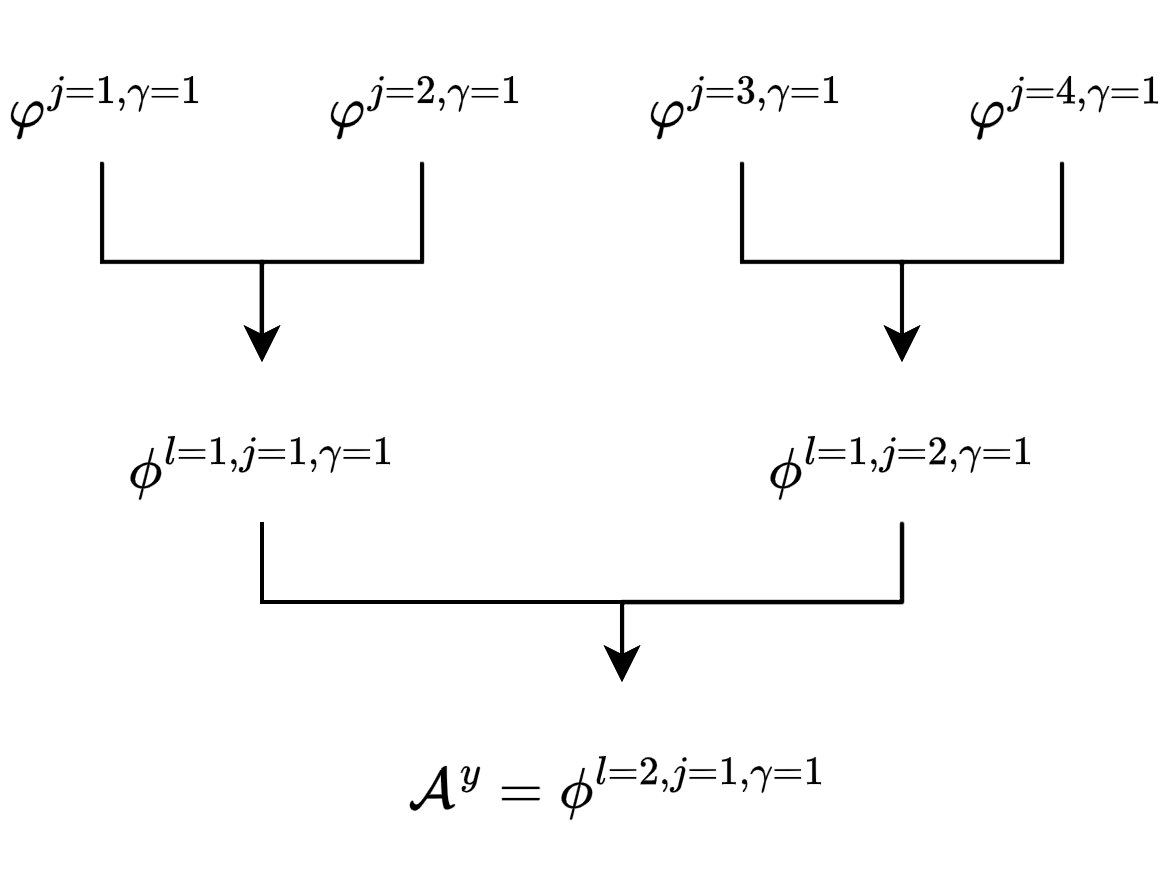
\includegraphics[width=0.6\textwidth]{matematicas/descomp_ht_rank_1}
	\caption{Ejemplo gráfico del proceso de construcción del tensor $\mathcal{A}^y$ a través de la descomposición \textit{HT}. Por simplicidad, estamos suponiendo que $r = 1$. Tenemos $L = 2$ capas o niveles}
	\label{img:diagrama_ht_simple}
\end{figure}

Veamos ahora este mismo diagrama, pero suponiendo que $r = 2$. Por tanto, en cada posición de cada nivel, tendremos dos tensores en vez de uno.

\begin{figure}[H]
	\centering
	\ajustarsubcaptions
	\begin{subfigure}{.5\textwidth}
		\centering
		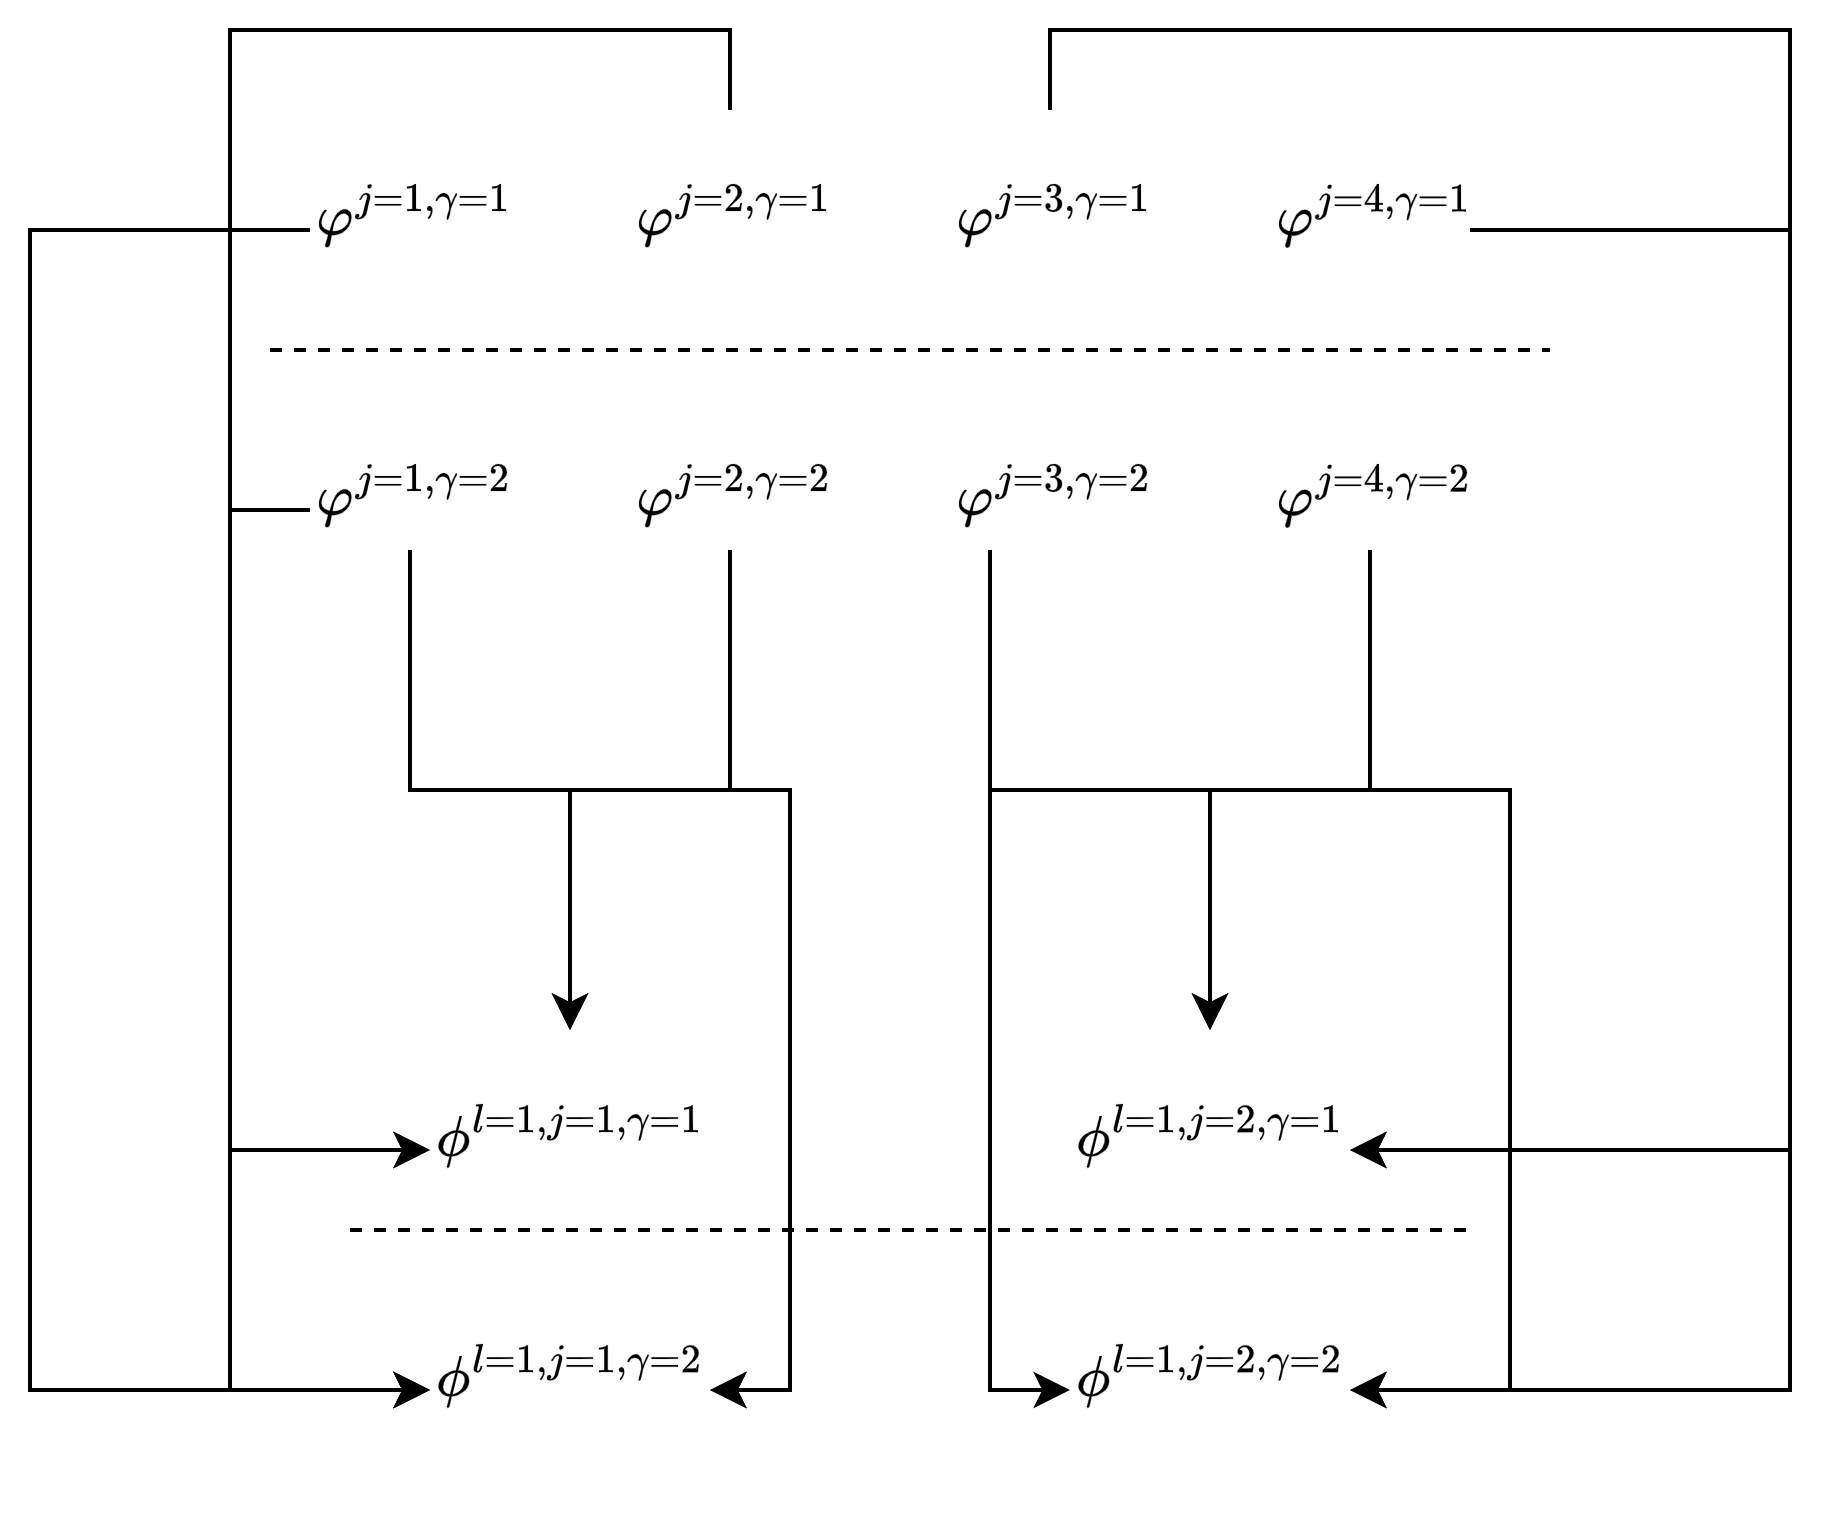
\includegraphics[width=0.9\linewidth]{matematicas/descomp_ht_rank_2_paso_1}
		\caption{Primer paso. En la construcción de cada tensor $\phi^{l, j, \gamma}$ participan cuatro vectores $\varphi^{j, \gamma}$}
	\end{subfigure}%
	\begin{subfigure}{.5\textwidth}
		\centering
		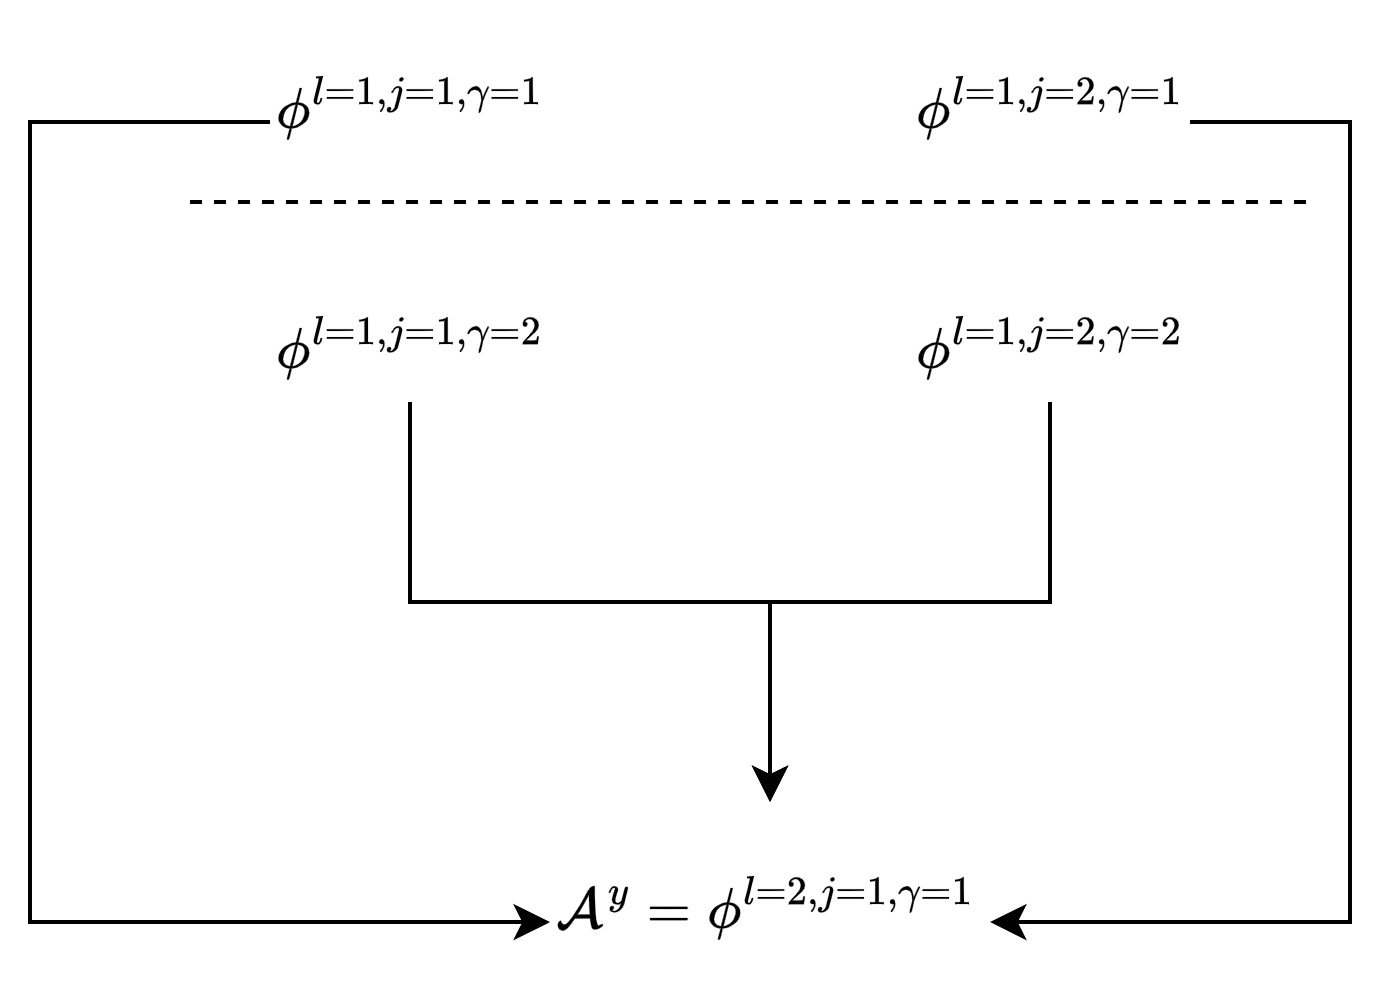
\includegraphics[width=0.9\linewidth]{matematicas/descomp_ht_rank_2_paso_2}
		\caption{Segundo paso. En la construcción del tensor $\mathcal{A}^y$ participan los cuatro tensores $\phi^{l=2, j, \gamma}$}
	\end{subfigure}
	\caption{Ejemplo gráfico del proceso de construcción del tensor $\mathcal{A}^y$ a través de la descomposición \textit{HT}. Hemos dividido el proceso de construcción en dos pasos. Ahora $r = 2$. Por lo tanto, en cada posición de cada capa, tenemos dos tensores. Seguimos teniendo $L = 2$ capas. }
	\label{img:diagrama_ht_complejo}
\end{figure}

La siguiente proposición nos muestra la relación de este modelo con el modelo \textit{CP}:

\begin{proposicion}
	La descomposición \textit{HT} es universal. Es más, extiende la descomposición \textit{CP}. Esto es, cualquier tensor que pueda expresarse como la descomposición \textit{CP} con rango \textit{CP} $Z$, admite una descomposición \textit{HT} con rangos $r_1 = r_2 = \ldots = r_{L - 1} = Z$
\end{proposicion}

\begin{proof}
	\todo{En la página 8 del paper se da una indicación de cómo se hace esto}
\end{proof}

\subsection{Número de parámetros del modelo} \label{msubs:parametros_modelo_ht}

Nuestro modelo viene dado por los siguientes parámetros:

\begin{itemize}
	\item Vectores iniciales:
	      \begin{equation}
		      \{\nv{\varphi^{j, \alpha}} \in \R^M: j \in \deltaset{N}, \alpha \in \deltaset{r_0}  \}
	      \end{equation}

	      Que suponen $M \cdot r_0 \cdot N$ coeficientes
	\item Pesos intermedios:

	      \begin{equation}
		      \{ a^{l, j, \gamma}_{\alpha} \in \R: l \in \deltaset{L-1}, j \in \deltaset{\frac{N}{2^l}}, \gamma \in \deltaset{r_l}, \alpha \in \deltaset{r_{l-1}} \}
	      \end{equation}

	      Con lo que aportan $\sum_{l = 1}^{L-1} r_{l-1} \cdot \frac{N}{2^l} \cdot r_l$ coeficientes.

	\item Pesos finales:

	      \begin{equation}
		      \{a^{L, y}_{\alpha}: y \in \deltaset{Y}, \alpha \in \deltaset{r_{L-1}} \}
	      \end{equation}

	      Por lo tanto, suponen $r_{L-1} \cdot Y$ coeficientes.
\end{itemize}

Es decir, que nuestro modelo tiene

\begin{equation}
	M \cdot r_0 \cdot N + \sum_{l = 1}^{L-1} (r_{l-1} \cdot \frac{N}{2^l} \cdot r_l ) +
	r_{L-1} \cdot Y
\end{equation}

coeficientes. Si asumimos que todos los rangos son iguales, $r := r_0 = \ldots = r_{L-1}$, entonces el número de coeficientes es:

\begin{equation}
	\begin{split}
		M \cdot r \cdot N + \sum_{l = 1}^{L-1} r^2 \cdot \frac{N}{2^l} + r \cdot Y &= M \cdot r \cdot N + N \cdot r^2 \cdot \frac{2^{L-1} - 1}{2^{L-1}} + r \cdot Y \longmapsto \ldots \\
		\ldots & \encima{\longmapsto}{L \mapsto \infty} M \cdot r \cdot N + N \cdot r^2 + r \cdot Y
	\end{split}
\end{equation}

donde hemos usado que:

\begin{equation}
	\sum_{l = 1}^{L-1} \frac{1}{2^l} = \frac{2^{L-1} - 1}{2^{L-1}}
\end{equation}

Podemos comprobar esto fácilmente:

\begin{proposicion}
	\begin{equation}
		\sum_{k = 1}^{N} \frac{1}{2^k} = \frac{2^N - 1}{2^N}; \dspace \forall N \in \N
	\end{equation}
\end{proposicion}

% Tengo hecha esta demostracion de forma directa en la pagina 49 de mis notas
\begin{proof}
	Procederemos por inducción. Veamos que la ecuación se verifica para $N = 1$:

	\begin{equation}
		\sum_{k = 1}^{1} \frac{1}{2^k} = \frac{1}{2} = \frac{2^1 - 1}{2^1}
	\end{equation}

	Supuesto que la ecuación se cumple para $N$, veamos si la ecuación se cumple para $N + 1$:

	\begin{equation}
		\begin{split}
			\sum_{k = 1}^{N+1} \frac{1}{2^k} &= \sum_{k = 1}^{N} (\frac{1}{2^k}) + \frac{1}{2^{N+1}} \encima{=}{\text{hip. ind.}} \ldots \\
			\ldots &= \frac{2^N - 1}{2^N} + \frac{1}{2^{N+1}} = \ldots \\
			\ldots &= \frac{2^{N+1} - 2 + 1}{2^{N+1}} = \ldots \\
			\ldots &= \frac{2^{N+1} - 1}{2^{N+1}}
		\end{split}
	\end{equation}
\end{proof}

\subsection{Relación entre la modelización y arquitecturas de aprendizaje automático}

El modelo \textit{HT} es el resultado de usar la descomposición \textit{HT} descrita en la ecuación \eqref{eq:descomposicion_ht} en nuestra función de puntuación \eqref{eq:puntuacion_general}. En esta sección, describiremos este modelo producido.

Como en el modelo \textit{CP}, el primer paso consiste en computar la capa de representación, $\{f_d(\nv{x_i}): d \in \deltaset{N}, \; i \in \deltaset{M}\}$. Esto genera $N \cdot M$ números reales, que serán transformados en las $L$ capas ocultas que producen la salida \eqref{eq:descomposicion_ht}.

Cada capa oculta se compone de una convolución $1 \times 1$ y un \textit{product pooling} con tamaño de ventana 2. En el modelo \textit{CP}, el \textit{product pooling} era global, colapsando las \textit{feature maps} a un único valor escalar. En este \textit{product pooling} reducimos el número de \textit{feature maps} a la mitad en cada paso.

Por lo tanto, tras las $L = log_2(N)$ capas ocultas, las $N$ \textit{feature maps} iniciales acaban siendo una única \textit{feature map}. Y con esto, acabamos con una lista de $r_{L - 1}$ coeficientes sobre los que aplicamos una última capa oculta, dada por la última ecuación de \eqref{eq:descomposicion_ht}.

Nuestra red realiza \textit{product pooling} con un tamaño de ventana 2, sin \textit{overlapping} gracias al hecho de que estamos combinando los tensores dos a dos, de forma contigua, como indican los ejemplos \customref{img:diagrama_ht_simple} y \customref{img:diagrama_ht_complejo}. Como muestra \cite{matematicas:descomposicion_ht}, podríamos haber escogido otra forma de combinar los tensores. Por ejemplo, combinando más de dos en cada paso. Esto produciría diferentes combinaciones de tamaños de ventana en el \textit{product pooling} y, por tanto, distintas profundidades.

En resumen, el funcionamiento de este modelo se puede observar en el siguiente diagrama:

\begin{figure}[H]
	\centering
	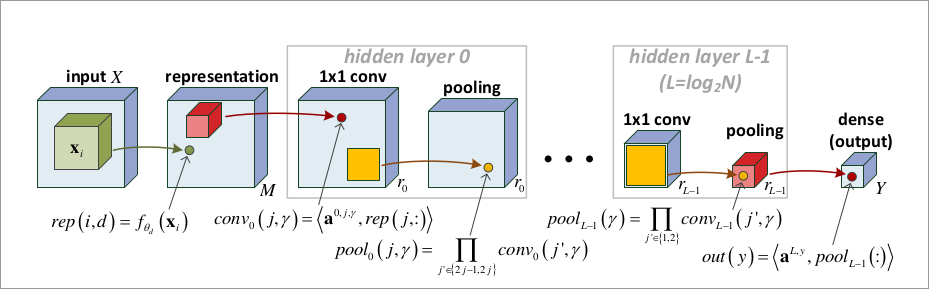
\includegraphics[width=0.8\textwidth]{matematicas/diagrama_paper_modelo_ht}
	\caption{Funcionamiento de nuestro modelo. Imagen extraída de \cite{matematicas:principal}}
\end{figure}
\todo{Sustituir este modelo por un diagrama realizado por mi}

\subsection{Compartición de coeficientes}

Al igual que ocurría en el modelo \textit{CP} \customref{subs:comparticion_parametros_cp}, nuestras convoluciones $1 \times 1$ son dependientes de la localización. En la práctica, en los modelos convolucionales los coeficientes de las convoluciones son independientes de la localización, lo que se conoce como \textbf{compartición de coeficientes}.

En el modelo \textit{HT} es muy fácil imponer la compartición de coeficientes, teniendo en cuenta los comentarios que hemos hecho en \customref{sec:modelo_ht}. Consideremos la ecuación de la capa $l$:

\begin{equation}
	\phi^{l, j, \gamma} := \sum_{\alpha = 1}^{r_{l-1}} a_{\alpha}^{l, j, \gamma} \cdot \phi^{l-1, 2j-1, \alpha} \otimes \phi^{l-1, 2j, \alpha}
\end{equation}

En $\phi^{l, j, \gamma}$:

\begin{itemize}
	\item $l$ indica la capa en la que nos encontramos
	\item $j$ indica la posición del tensor en la capa $l$
	\item $\gamma$ indica con qué tensor trabajamos en la posición $j$, porque podemos tener más de un tensor en cada posición (cuando $r_l > 1$)
\end{itemize}

Por lo tanto, los coeficientes $\nv{a^{l, j, \gamma}} := (a^{l, j, \gamma}_1, \ldots, a^{l, j, \gamma}_{r_{l-1}})$ no deberían depender de la posición $j$. Con esto, para imponer la compartición de coeficientes basta con hacer:

\begin{equation}
	\nv{a^{l, 1, \gamma}} = \nv{a^{l, 2, \gamma}} = \ldots = \nv{a^{l, N/2^l, \gamma}} =: \nv{a^{l, \gamma}}; \dspace \forall l \in \doubledeltaset{0}{L - 1} \dspace \forall \gamma \in \deltaset{r_l}
\end{equation}

Como ocurría en \customref{subs:comparticion_parametros_cp}, esta imposición provoca que nuestro modelo pierda la universalidad. Esto es, nuestro modelo no puede representar cualquier tensor, independientemente de los valores de $L$ o $r_l$. Aunque en este caso, los tensores que podemos generar con la compartición de parámetros no están limitados a ser simétricos, como en el caso \textit{CP}. Esto ya es un primer indicativo de que el modelo \textit{HT} es más expresivo que el modelo \textit{CP}.

\section{Comparativa del número de coeficientes de cada modelo}

El número de coeficientes de cada modelo es un aspecto central en nuestro estudio. Por tanto, comparamos ahora la diferencia en dicho número de coeficientes de cada modelo.

Para ello, consideramos el hecho de que \textit{HT} es una extensión de \textit{CP}. Por lo tanto, un modelo \textit{CP} con cierto valor de $Z$ tiene  $N \cdot M \cdot Z + Z \cdot Y$ coeficientes que especificar (\customref{msubsec:parametros_modelo_cp}). Si queremos implementar el resultado de dicho modelo con un modelo \textit{HT}, deberemos considerar $r = Z$ y por ello, tendremos $N \cdot M \cdot Z + N \cdot Z^2 \cdot \frac{2^{L-1} - 1}{2^{L-1}} + Z \cdot Y$ (\customref{msubs:parametros_modelo_ht}).

Por lo tanto, la diferencia en número de coeficientes viene dada por:

\begin{equation}
	Z^2 \cdot \frac{2^{L-1} - 1}{2^{L-1}} \encima{\longmapsto}{L \mapsto \infty} N \cdot Z^2
\end{equation}

Es decir, que podemos implementar cualquier modelo \textit{CP} con un modelo \textit{HT}, pero tenemos una \textbf{penalización cuadrática} en el número de coeficientes que tenemos que aprender.

Esto puede hacernos pensar que el modelo \textit{CP} es mejor, porque requiere menos coeficientes. Sin embargo, no olvidemos que estamos estudiando el caso en el que, dado un modelo \textit{CP}, lo replicamos con un modelo \textit{HT}. Hay varios puntos
que no tenemos en cuenta:

\begin{itemize}
	\item Dado un modelo \textit{HT} cualquiera, ¿podemos implementarlo con un modelo \textit{CP}? De ser así, ¿cuál sería la penalización en número de coeficientes?
	\item ¿Existen funciones implementables por un modelo \textit{HT} que no lo sean por un modelo \textit{CP}?
\end{itemize}

Respecto a la segunda pregunta, ya sabemos que en el caso de imponer compartición de coeficientes, el modelo \textit{HT} puede representar ciertos $\mathcal{A}^y$ no simétricos que el modelo \textit{CP} será incapaz de representar.

Responderemos a la primera pregunta con los dos resultados principales del trabajo. Pero en resumen, sí podremos representar el resultado de un modelo \textit{HT} con un modelo \textit{CP}, pero la penalización será exponencial.
